% Created 2025-03-08 Sat 17:10
% Intended LaTeX compiler: pdflatex
\documentclass[11pt]{article}
\usepackage[utf8x]{inputenc}
\usepackage[T1]{fontenc}
\usepackage{graphicx}
\usepackage{longtable}
\usepackage{wrapfig}
\usepackage{rotating}
\usepackage[normalem]{ulem}
\usepackage{amsmath}
\usepackage{amssymb}
\usepackage{capt-of}
\usepackage{hyperref}
\usepackage{minted}
\usepackage{parskip}
\usepackage[labelformat=simple]{subcaption}
\renewcommand\thesubfigure{(\alph{subfigure})}
\setcounter{secnumdepth}{3}
\author{Raghav B. Venkataramaiyer}
\date{Feb '25}
\title{Practice Questions for Graph Theory\\\medskip
\large Representation, Search Algorithms, and Variants for Problem Solving}
\hypersetup{
 pdfauthor={Raghav B. Venkataramaiyer},
 pdftitle={Practice Questions for Graph Theory},
 pdfkeywords={},
 pdfsubject={},
 pdfcreator={Emacs 29.4 (Org mode 9.6.24)}, 
 pdflang={English}}
\begin{document}

\maketitle

\section{Graph Representations}
\label{sec:org2912b19}

\subsection{Fundamentals}
\label{sec:org25f41f3}


\paragraph*{Question 1}
\label{sec:org48ec970}
Are graphs useful in real world?  Support your answer
with examples from your domain.

\paragraph*{Question 2}
\label{sec:orgc48ae40}
What is the difference between adjacency list and
adjacency matrix?  Cite real world examples of usage.

\emph{Hint:} List is compact, whereas Matrix is detailed.
List makes more sense in sparse graphs, and Matrix in
dense ones.

\paragraph*{Question 3}
\label{sec:orga3771f0}
If \(G(V,M)\) represents a given graph \(G\) with a set of
vertices \(V\) and adjacency matrix \(M\), what is the
significance of a transpose graph
\(G^{\top}(V,M^{\top})\)?  Cite examples from your domain
for emphasis.

\emph{Hint:} The edges in \(G^{\top}\) are reversed when
compared against those in \(G\).  (See also: 
\S~\ref{sec:transpose-graph})

\paragraph*{Question 4}
\label{sec:orgd03eb36}
Comment on the nature of graph \(G(V,M+M^{\top})\) where
\(M\) is a square matrix with empty diagonals.

\emph{Hint:} If \(M\) consists of forward edges, then it
follows that \(M^{\top}\) corresponding are reverse
edges; hence \(M+M^{\top}\) consists of bi-directional
edges.  (See also: 
\S~\ref{sec:transpose-graph})

\subsection{Vertex Insertion}
\label{sec:org8908407}
\paragraph*{Question}
\label{sec:org1209108}

\(\overline{\mathit{ABCD}}\) is a closed quadrilateral.
A new vertex \(E\) is introduced between \(B\) and \(C\).
Show the adjacency lists before and after the
introduction of \(E\).  Hence, write an algorithm/
pseudocode in order to introduce a new vertex between
an existing edge.

\paragraph*{Interpretation}
\label{sec:org3e6b2bc}
Given a closed quadrilateral
\(\overline{\mathit{ABCD}}\), the adjacency list in
1-indexed format is given as:

\begin{verbatim}
V = [A, B, C, D]
Adj = [[2, 4],                  # 1 is connected to 2 and 4
       [1, 3],                  # 2 is connected to 1 and 3
       [2, 4],                  # and so forth
       [1, 3]]
\end{verbatim}

Here the edge \(\overline{\mathit{BC}}\) is defined in
two entries of the adjacency list, \emph{i.e.} as vertex \texttt{3}
in \texttt{Adj[2]} and vertex \texttt{2} in \texttt{Adj[3]}.

\paragraph*{Solution}
\label{sec:org0d5868c}

In order to introduce a new vertex \(E\) between edge
\(\overline{\mathit{BC}}\),

\subparagraph*{Step 1}
\label{sec:org14d35fb}
Append vertex \(E\) to the vertex list \(V\) and get its
index.

\begin{verbatim}
V = [A, B, C, D, E]             # Add E as V[5]
\end{verbatim}

\subparagraph*{Step 2}
\label{sec:orgf0437b0}
Remove the edge  \(\overline{\mathit{BC}}\)
\begin{verbatim}
V = [A, B, C, D, E]
Adj = [[2, 4],
       [1],                     # remove 3 from Adj[2]
       [4],                     # remove 2 from Adj[3]
       [1, 3],
       []]                      # add empty Adj[5]
\end{verbatim}

\subparagraph*{Step 3}
\label{sec:org50e54e7}
Add edges \(\overline{\mathit{BEC}}\)
\begin{verbatim}
V = [A, B, C, D, E]
Adj = [[2, 4],
       [1, 5],                  # add 5 to Adj[2]
       [4, 5],                  # add 5 to Adj[3]
       [1, 3],
       [2, 3]]                  # add 2, 3 to Adj[5]
\end{verbatim}

\subparagraph*{Algorithm}
\label{sec:org205e505}

To introduce a vertex \(W\) between an edge \((u,v)\),

\begin{verbatim}
GRAPH_ADD_VERTEX_BW(G,W,u,v) :
  w = G.V.append(W)             # Insert W into list of
                                # vertices and store the
                                # last appended index.

  G.Adj[u].remove(v)            # Remove v from Adj[u]
  G.Adj[v].remove(u)            # Remove u from Adj[v]

  G.Adj[u].append(w)            # Append w into Adj[u]
  G.Adj[v].append(w)            # Append w into Adj[v]

  G.Adj[w].append(u)            # Append u into Adj[w]
  G.Adj[w].append(v)            # Append v into Adj[w]
\end{verbatim}

\textbf{PS}: Here, \(W\) in uppercase refers to a variable
(\emph{i.e.} vertex information like coordinates of a point
etc.) that needs to appended into the list of verts
\(G.V\). And \((u,v)\) represent the indices of the pair of
verts that constitute and edge.  We are interested in
the Adjacency List (as required by the question,) hence
the use of \(G.Adj\)

\subsection{Transpose Graph}
\label{sec:transpose-graph}
\paragraph*{Question}
\label{sec:org5637b57}
Given a graph \(G(V,M)\), \(M\) being the adjacency matrix.
A transpose graph would be the one with same set of
vertices, but a transposed adjacency matrix, \emph{i.e.}
\(G^{\top}(V,M^{\top})\).  What does a transpose graph
represent?  Illustrate with a drawing to support your
answer.

\paragraph*{Interpretation}
\label{sec:org44ce834}
Recall that,
\begin{enumerate}
\item In an adjacency matrix \(A\), the component at
\(i^{\text{th}}\) row, and \(j^{\text{th}}\) column is
given as \(a_{ij}\) and it represents whether the edge
\(v_{i}\to v_{j}\) exists.
\item A transpose graph \(G^{\top}(V,M^{\top})\) would be
any different, \emph{iff} \(M\ne M^{\top}\).  In other
words, if \(G\) is a directed graph.
\item The components in the transposed matrix are mirrored
across the diagonal.  Hence, if \(B = A^{\top}\), then
\(b_{ij} = a_{ji}\).
\end{enumerate}

\paragraph*{Solution}
\label{sec:org3ec361b}

Each edge \(v_{i}\to v_{j}\) in \(G\), transforms to
\(v_{j}\to v_{i}\) in the transpose graph \(G^{\top}\).
In other words, the edges are reversed.

This would be any different, only in case of a directed
graph.  Since for an undirected graph \(M=M^{\top}\).
Hence, the transpose graph \(G^{\top}(V,M^{\top})\)
represents \(G(V,M)\) with edges reversed.

\paragraph*{Illustration}
\label{sec:orgd5bf782}

\begin{align*}
  M = \begin{bmatrix}
    0&1&0\\0&0&1\\1&0&0
  \end{bmatrix}\quad M^{\top} = \begin{bmatrix}
    0&0&1\\1&0&0\\0&1&0
  \end{bmatrix}\quad M+M^{\top} = \begin{bmatrix}
    0&1&1\\1&0&1\\1&1&0
  \end{bmatrix}
\end{align*}

\begin{figure}[htbp]
\centering
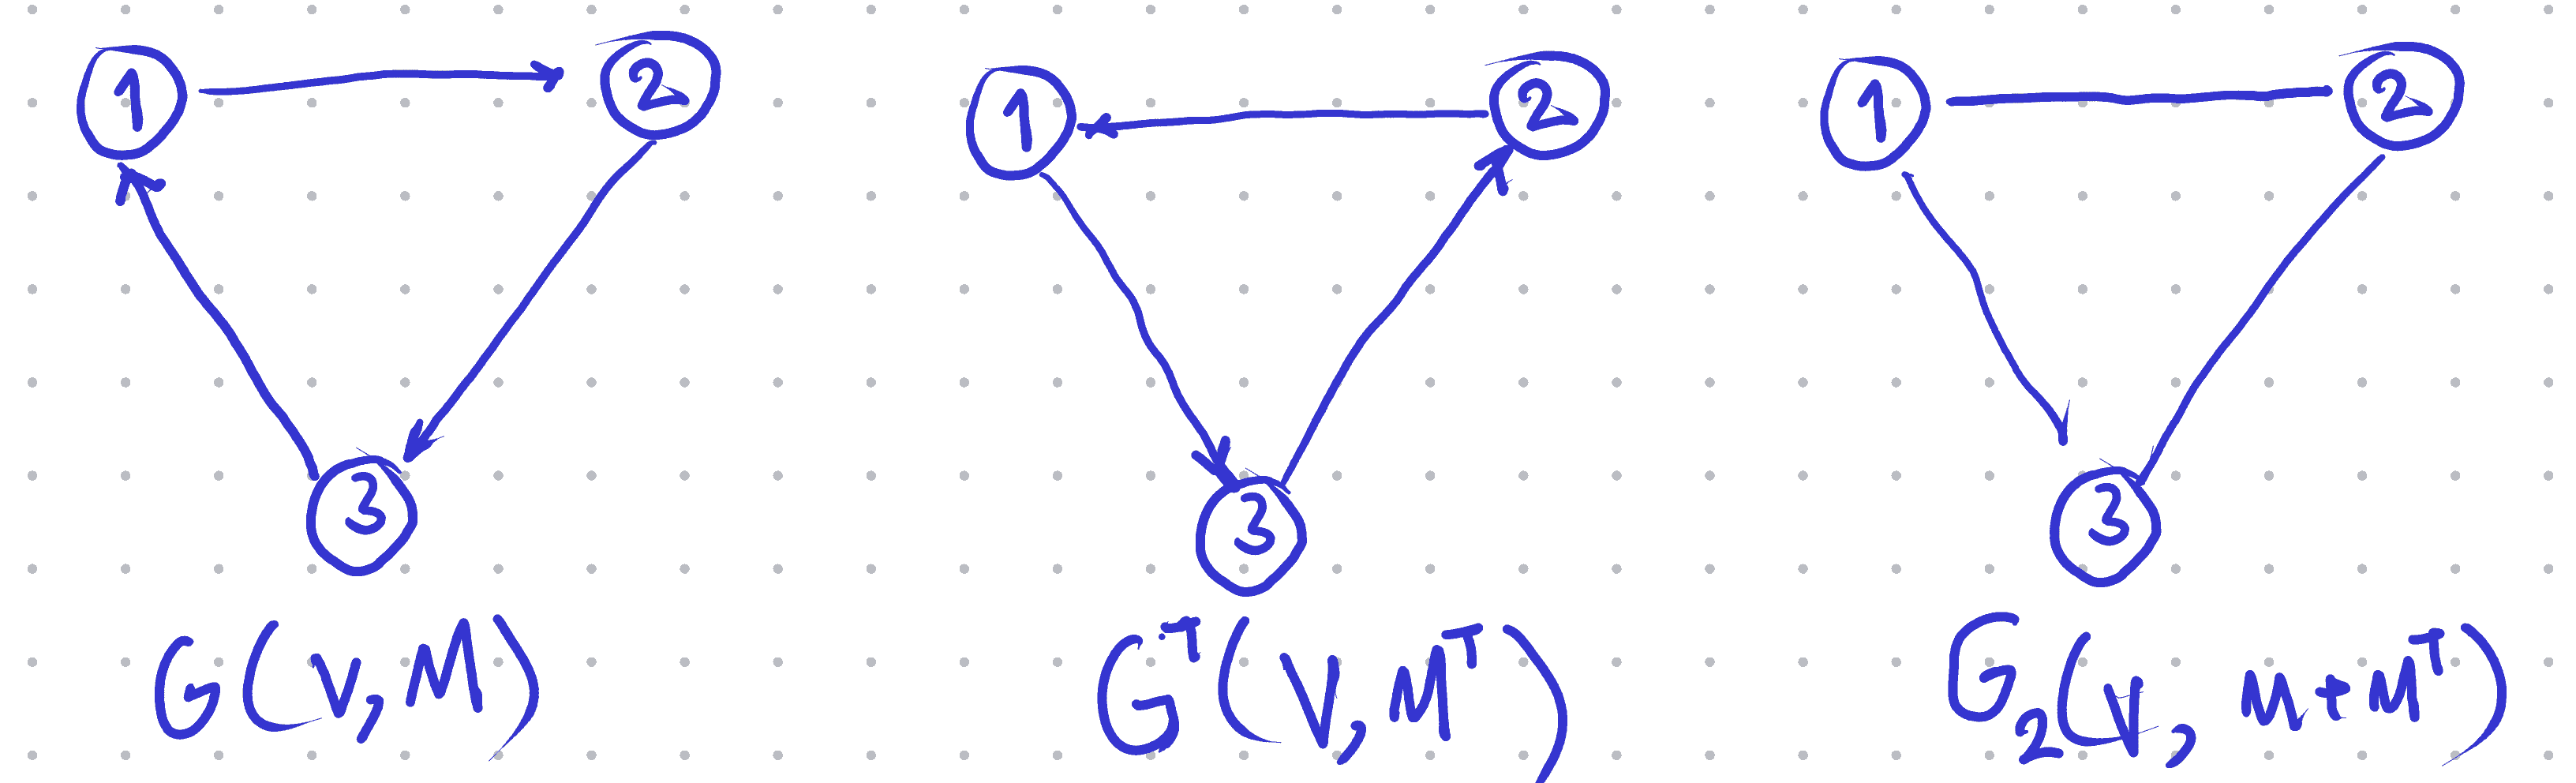
\includegraphics[width=.9\linewidth]{images/transpose-graphs.png}
\caption{\label{fig:transposeGraph}Graph and its Transpose}
\end{figure}


\subsection{(In/Out)-degree}
\label{sec:org4c57af4}

\paragraph*{Question}
\label{sec:org930561b}
What is the average in-degree of a graph \(G(V,E)\),
where \(E\) is the set of edges in \(G\)?

\paragraph*{Solution}
\label{sec:org8daa2e0}
In-degree of a vertex is defined as the number of
edges leading onto itself.

Let \(d_{\mathrm{in}}(v)\) represent the in-degree of
vertex \(v\).  Then the average in-degree is given as the
sum of in-degrees divided by the size of number of
verts,

\begin{align*}
  \mathbb{E}[d_{\mathrm{in}}(v)]
  &= \frac{\sum_{v\in V}d_{\mathrm{in}}(v)} {|V|}
\end{align*}

Intuitively speaking, the sum of all in-degrees is the
same as the number of edges. Hence,

\begin{align*}
  \mathbb{E}[d_{\mathrm{in}}(v)]
  &= \frac{|E|} {|V|}
\end{align*}

\paragraph*{In further detail}
\label{sec:org94bddb6}

In-degree of a vertex is the same as counting the
non-zeros in one (specific) column of an adjacency
matrix representation \(M\) for the set of edges \(E\).

Similarly, the sum \(\sum_{v\in V}d_{\mathrm{in}}(v)\) is
equivalent to

\begin{itemize}
\item Counting the non-zeros for every the column of \(M\),
\item \emph{i.e.} Counting all the non-zeros in \(M\),
\item \emph{i.e.} The number of edges.
\end{itemize}

Hence,

\begin{align*}
  \sum_{v\in V} d_{\mathrm{in}}(v)
    &= |E|
\end{align*}



\subsection{Representation}
\label{sec:org94cc111}

\paragraph*{Question}
\label{sec:org10e36c4}
Provide an adjacency list as well as the adjacency matrix
representation for trees A and B in the following figure.

\begin{figure}[!h]
\centering
\begin{minipage}{0.4\textwidth}
\centering
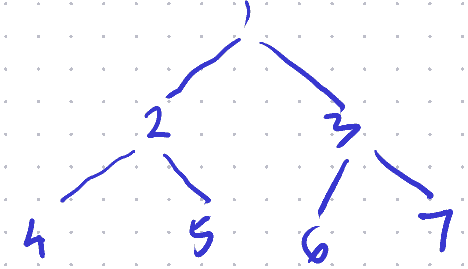
\includegraphics[width=\linewidth]{./images/treeA.png}
\subcaption{\label{fig:treeA} Tree A}
\end{minipage}
\begin{minipage}{0.5\textwidth}
\centering
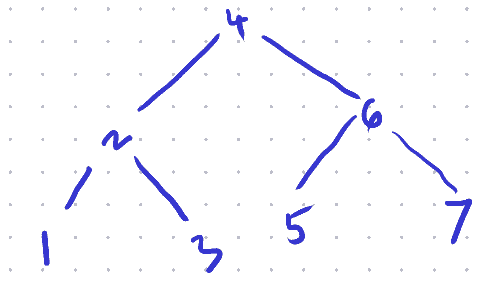
\includegraphics[width=\linewidth]{./images/treeB.png}
\subcaption{\label{fig:treeB} Tree B}
\end{minipage}
\end{figure}

\paragraph*{Solution}
\label{sec:orgb14f9e1}

\subparagraph*{Tree A}
\label{sec:org07614f1}
\begin{verbatim}
Adj = [[2 3] 
       [1 4 5] 
       [1 6 7] 
       [2]
       [2]
       [3]
       [3]]

M = [[0 1 1 0 0 0 0]
     [1 0 1 1 0 0 0]
     [1 0 0 0 1 1 0]
     [0 1 0 0 0 0 0]
     [0 1 0 0 0 0 0]
     [0 0 1 0 0 0 0]
     [0 0 1 0 0 0 0]]
\end{verbatim}

\subparagraph*{Tree B}
\label{sec:org5d0634f}
\begin{verbatim}
Adj = [[2]
       [1 3 4]
       [2]
       [2 6]
       [6]
       [4 5 7]
       [6]]
M = [[0 1 0 0 0 0 0]
     [1 0 1 1 0 0 0]
     [0 1 0 0 0 0 0]
     [0 1 0 0 0 1 0]
     [0 0 0 0 0 1 0]
     [0 0 0 1 1 0 1]
     [0 0 0 0 0 1 0]]
\end{verbatim}

\subparagraph*{PS}
\label{sec:org69d9c2a}
The Adjacency matrix of Tree B is bi-symmetric.

\section{Elementary Algorithms}
\label{sec:org845571d}

\subsection{Fundamentals}
\label{sec:orgf27a83c}

\paragraph*{Question 1}
\label{sec:orgb90c209}

Cite examples to highlight the difference between when
and why to prioritise the use of BFS in stead of DFS,
and vice-versa.

\paragraph*{Question 2}
\label{sec:org148745a}

What operations are performed while visiting a vertex
\(v\) during BFS.  How are they different from visiting a
vertex \(v\) during DFS?

\emph{Hint:} One iteration of while loop is a visit during
BFS, whereas visit in a DFS finishes only after all
successors have been visited.

\emph{PS:} The answer to this question is also the
difference between stacked and queued operations in
general.

\paragraph*{Question 3}
\label{sec:org70450cb}

Visiting a vertex in BFS assigns three vertex
properties.  Describe them highlighting their
importance in problem solving in general.

\emph{Hint:} Discovery time is also the distance from
source; and following the parent is the shortest path
to source.

\paragraph*{Question 4}
\label{sec:org7ffd991}

How is DFS useful in real world?  Emphasise the
significance of discovery and finish times in your
example?

\paragraph*{Question 5}
\label{sec:org9cbaaad}

At any instant, during the DFS, how does the colour of
a node, help determining the edge classification?

\emph{Hint:} See \href{https://docs.google.com/presentation/d/14PY-Sc50QsFxdUqZk7GlYVwwEXzO38rg9z9KKx5ti0k/edit\#slide=id.g32a7028b731\_0\_422}{this slide}

\paragraph*{Question 6}
\label{sec:orgdf69cab}

How can DFS be used to detect cycles in a graph?
Comment.

\paragraph*{Question 7}
\label{sec:org48f1b74}

How can parenthesis structure of a DFS help determine
dependencies and relationships?

\emph{Variants:}

\begin{enumerate}
\item A project is subdivided into tasks, and it has been
understood that some tasks are dependent upon
others.  How would you determine if one task must be
completed before another?  Write an algorithm/
pseudocode for the same.

\emph{Hint:} ``One task must be completed before another''
implies an order.

\item Given a large family database, with parent-child
relationships between individuals, how would you
determine if at all related (directly), Jaspreet is
ancestor/descendant of Dilraj?

\emph{Hint:} Parenthesis structure exhibits direct
relationships.
\end{enumerate}

\emph{See Also:} 
\S~\ref{sec:dfs-parenthesis-structure}

\subsection{BFS}
\label{sec:orgc32bee0}

\paragraph*{Question}
\label{sec:orgf01a2f3}

\begin{figure}[htbp]
\centering
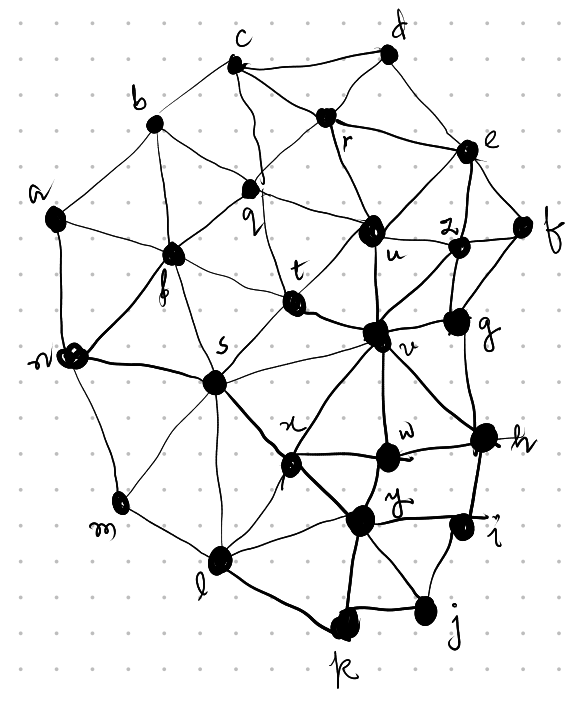
\includegraphics[width=0.5\linewidth]{images/graphA.png}
\caption{\label{fig:graphA}Graph A}
\end{figure}

With reference to Graph A (see
Fig~\ref{fig:graphA}) \textbf{Determine algorithmically},

\begin{enumerate}
\item The shortest path weight \(\delta(u,j)\) for the pair
\((u,j)\) of vertices.
\item A shortest path between the pair \((u,j)\) of
vertices.
\item All shortest-paths originating from vertex \(u\).
\end{enumerate}

\begin{figure}[htbp]
\centering
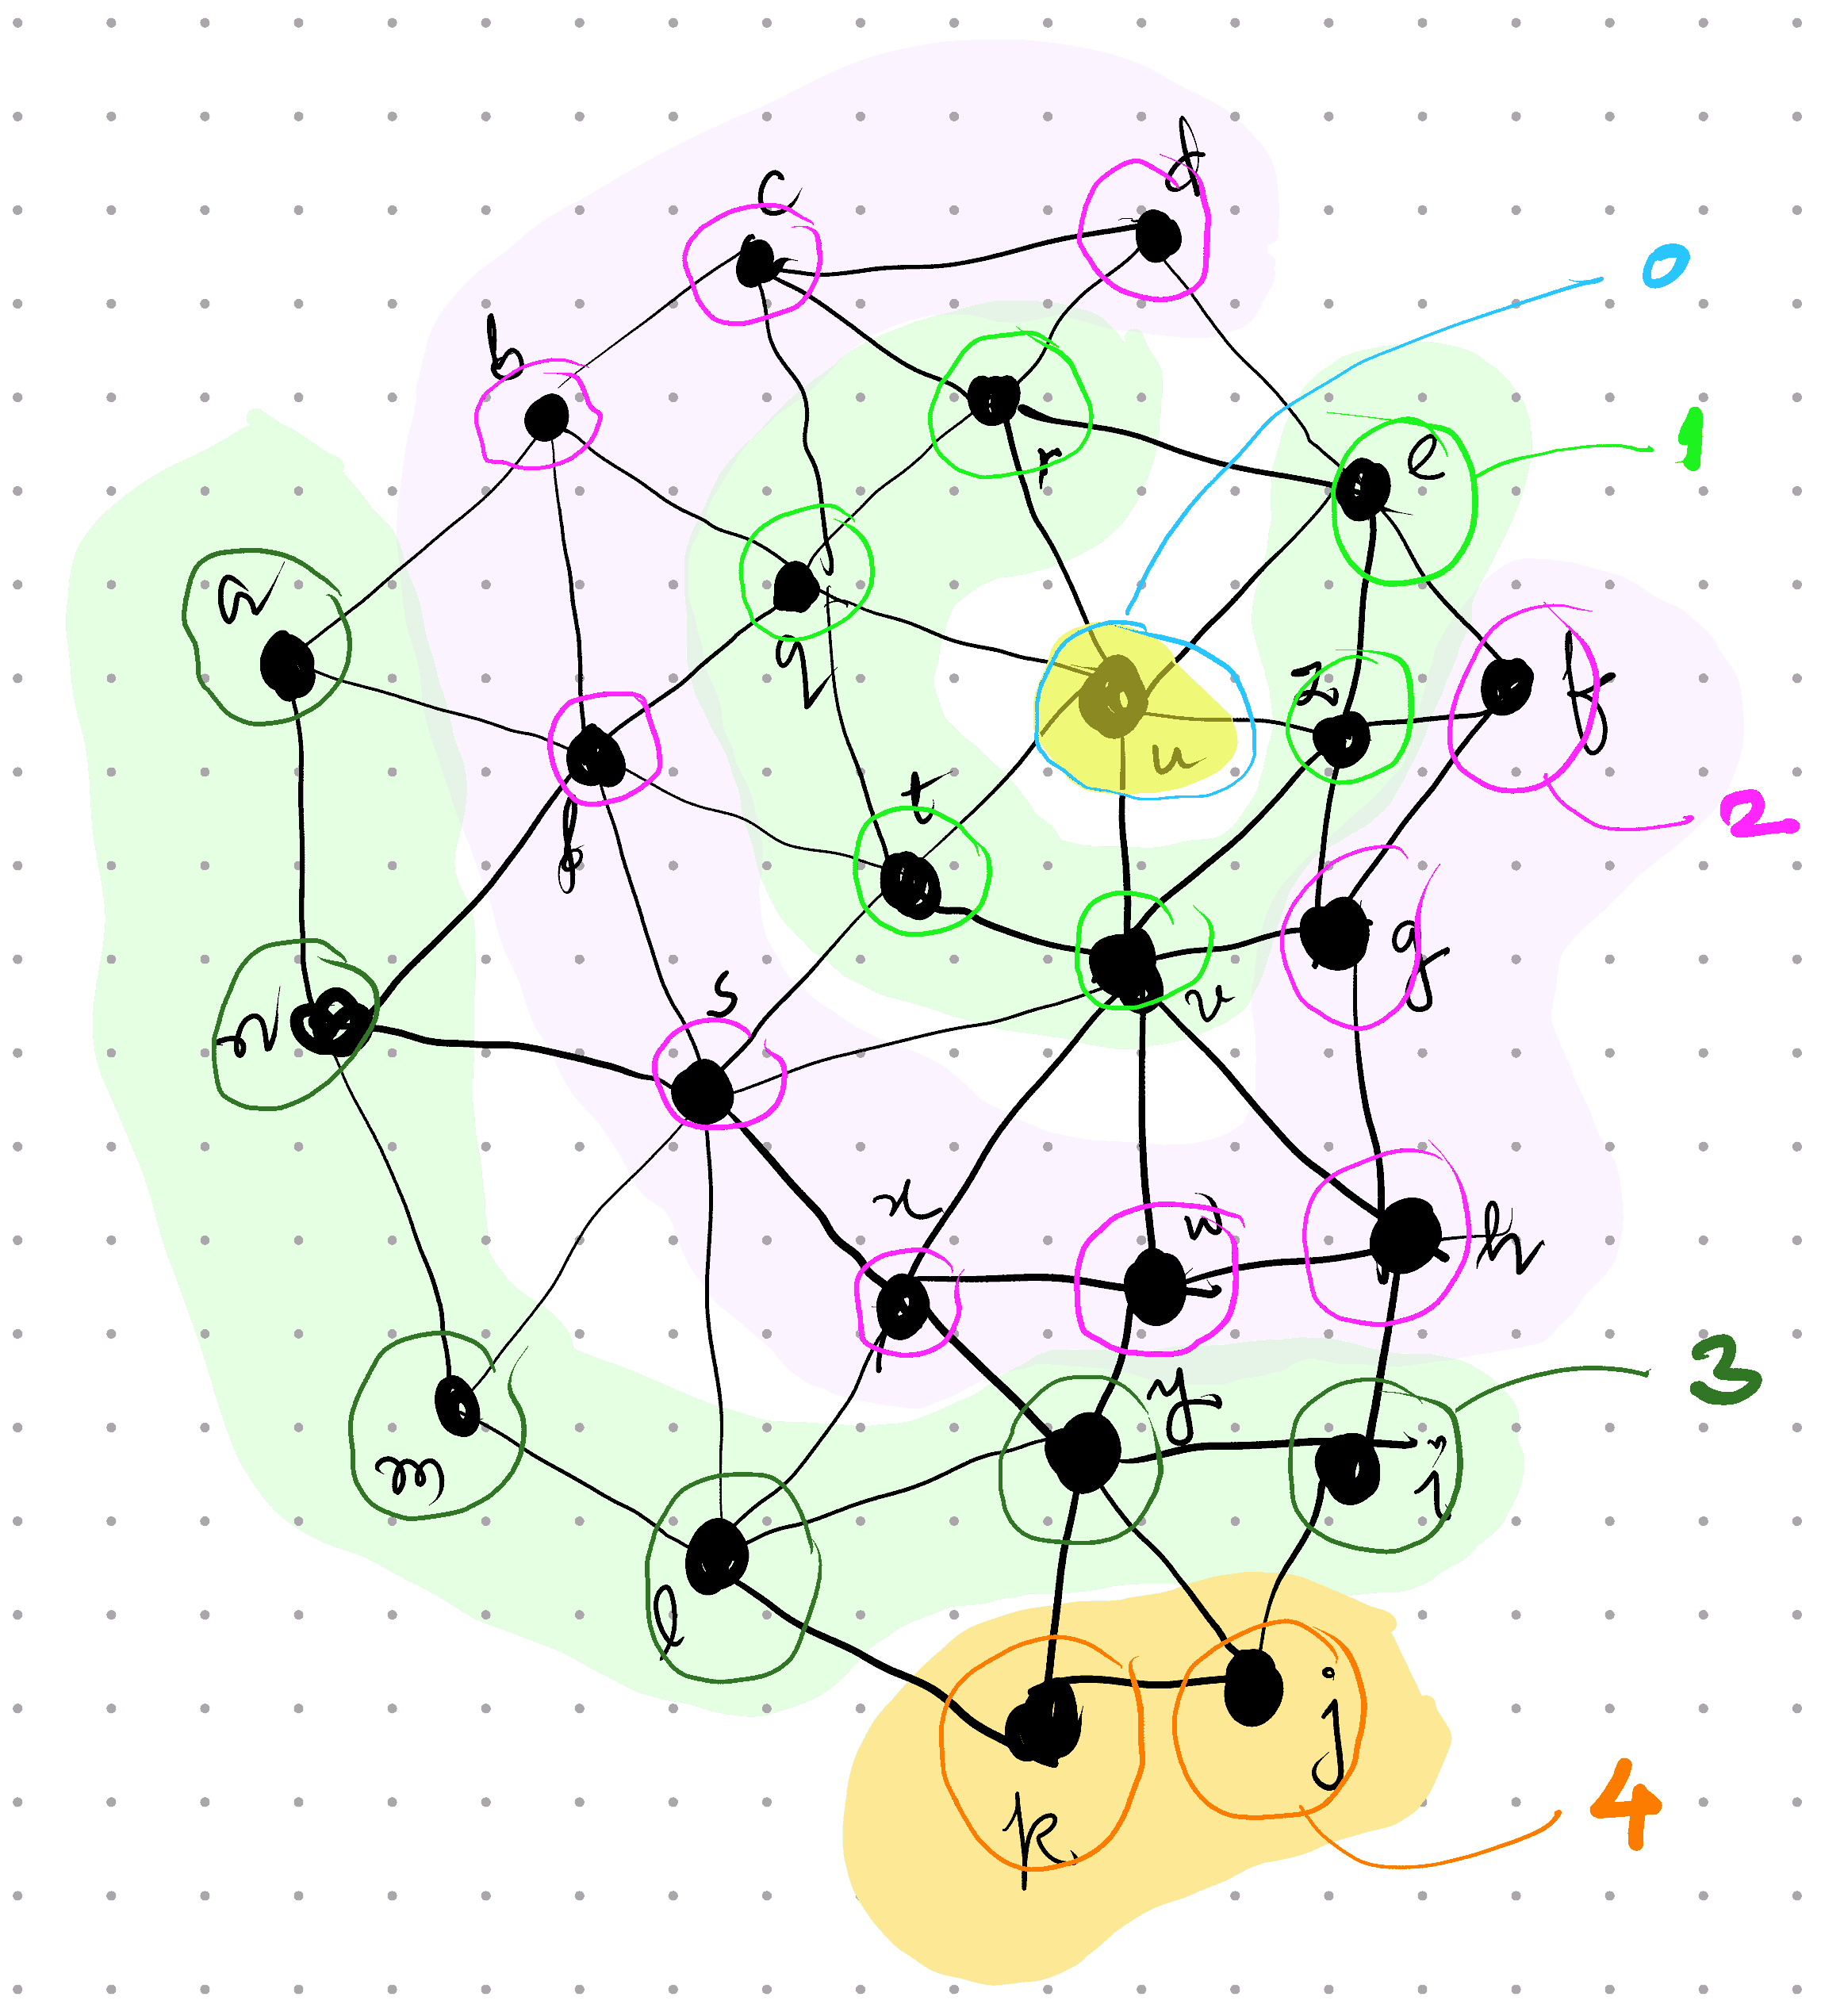
\includegraphics[width=\linewidth]{images/bfsOnGraphA.png}
\caption{\label{fig:bfsOnGraphA}BFS on Graph A}
\end{figure}
\paragraph*{Key Insight}
\label{sec:org4e87020}
All the three questions here speak about a shortest
path originating from vertex \(u\).  This is a uniformly
weighted undirected graph, \emph{i.e.} all edges are equally
weighted.  The solution for shortest path will follow a
BFS in such a case.

\paragraph*{Solution}
\label{sec:org6762907}
\begin{enumerate}
\item Running a BFS on the graph gives us the figure, ``BFS
on Graph A'' (Fig~\ref{fig:bfsOnGraphA})
upon termination.
\item The numbers marked are discovery times of the nodes \\[0pt]
\(v\cdot d \ \forall v\in V\).
\item For part (1) the shortest path weight is given as
\(\delta(u,j) = j\cdot d - u\cdot d\).  Computing from
the figure, \(\delta(u,j) = 4-0 = 4\).
\item For part (2) we may pick any one path such that each
successive node is from successive level.  \emph{i.e.}
one of,
\begin{enumerate}
\item \(\langle u,v,h,i,j\rangle\),
\item \(\langle u,v,w,y,j\rangle\), or
\item \(\langle u,v,x,y,j\rangle\).
\end{enumerate}

Recall, that only one of these is, and not all of
them are, the required shortest path (\emph{i.e.}
discovered in one run).

\item For part (3), a BFS tree is required.  It's been
left that upon the reader to exercise and present as
necessary.  An easy way out would be to use the
adjoining graph
(Fig~\ref{fig:bfsOnGraphA}) and
additionally mark each connection from ``parent'' to
``child'' as descended during the BFS.  Note that the
arrow would be a manifestation of line \texttt{v.PI = u} in
the algorithm \href{https://docs.google.com/presentation/d/14PY-Sc50QsFxdUqZk7GlYVwwEXzO38rg9z9KKx5ti0k/edit\#slide=id.g32a7028b731\_0\_60}{(link to the slide)}.  Recall that
there may be only one parent to a child, not many,
and that the discovery time of the parent is always
less than that of the child.
\end{enumerate}

\subsection{DFS}
\label{sec:org8d2e1a9}

\paragraph*{Question}
\label{sec:org0cbff93}
Given that there are 10 courses in a programme, and
corresponding pre-requisites are listed as under,
\textbf{determine algorithmically} If the programme may be
completed successfully by a candidate?

\begin{enumerate}
\item depends upon 2 and 3;
\item depends upon 3 and 4;
\item depends upon none;
\item depends upon none;
\item depends upon 4 and 6;
\item depends upon none;
\item depends upon 5 and 8;
\item depends upon 4, 6 and 10;
\item depends upon 2, 4 and 8;
\item depends upon 6 and 9.
\end{enumerate}

\paragraph*{Key Insight}
\label{sec:org5a39456}
We define a relationship \(u\to v\) if course \(u\) depends
upon \(v\) (\emph{i.e.} if course \(v\) is a pre-requisite of
course \(u\)).  Then we get a dependency graph (\emph{i.e.} a
directed graph where relationship is defined when the
parent is dependent upon the child).

A topological order \(T\equiv\langle v_{1},\ldots,v_{k}
\rangle\) of such a graph means that all ancestors of
\(v_{i}\) have been listed before \(v_{i}\) itself \(\forall
v_{i}\in V\).  In simple words, the topological order is
one possible order of courses to complete the
programme.

However, the topological order is not always possible.
From \href{https://docs.google.com/presentation/d/14PY-Sc50QsFxdUqZk7GlYVwwEXzO38rg9z9KKx5ti0k/edit\#slide=id.g32a7028b731\_0\_377}{our slides}, we know that topological order is
defined only for a directed acyclic graph (DAG).
\textbf{Hence, one may complete the programme iff the
dependency graph is acyclic.}

And \textbf{a graph is acyclic if and only if there are no
back edges.}

\paragraph*{Solution}
\label{sec:orgae5a43e}
\begin{enumerate}
\item Run a DFS on Dependency Graph;
\item Maintain a list \(T\) for Topological Order;
\item Upon finishing the visit to a node, insert the node
to the front of the list;
\item Exit ``abnormally,'' if encountered a ``back edge.''
\end{enumerate}

If exited abnormally, the graph has a cycle; and the
programme can not be completed successfully.

Otherwise, the graph is acyclic, and \(T\) contains an
order of courses that successfully completes the
programme.

In figure ``DFS on Dependency Graph,''
(Fig~\ref{fig:dfsOnDependencyGraph}) nodes
have been mentioned with discovery and finish times;
and edges have been labelled as B,C,F,T for back edges,
cross edges, forward edges and tree edges respectively.

The algorithm terminated upon visiting the edge \(9\to
8\) which is a back edge (labelled B).

\textbf{Hence the programme can not be completed.}
\begin{figure}[htbp]
\centering
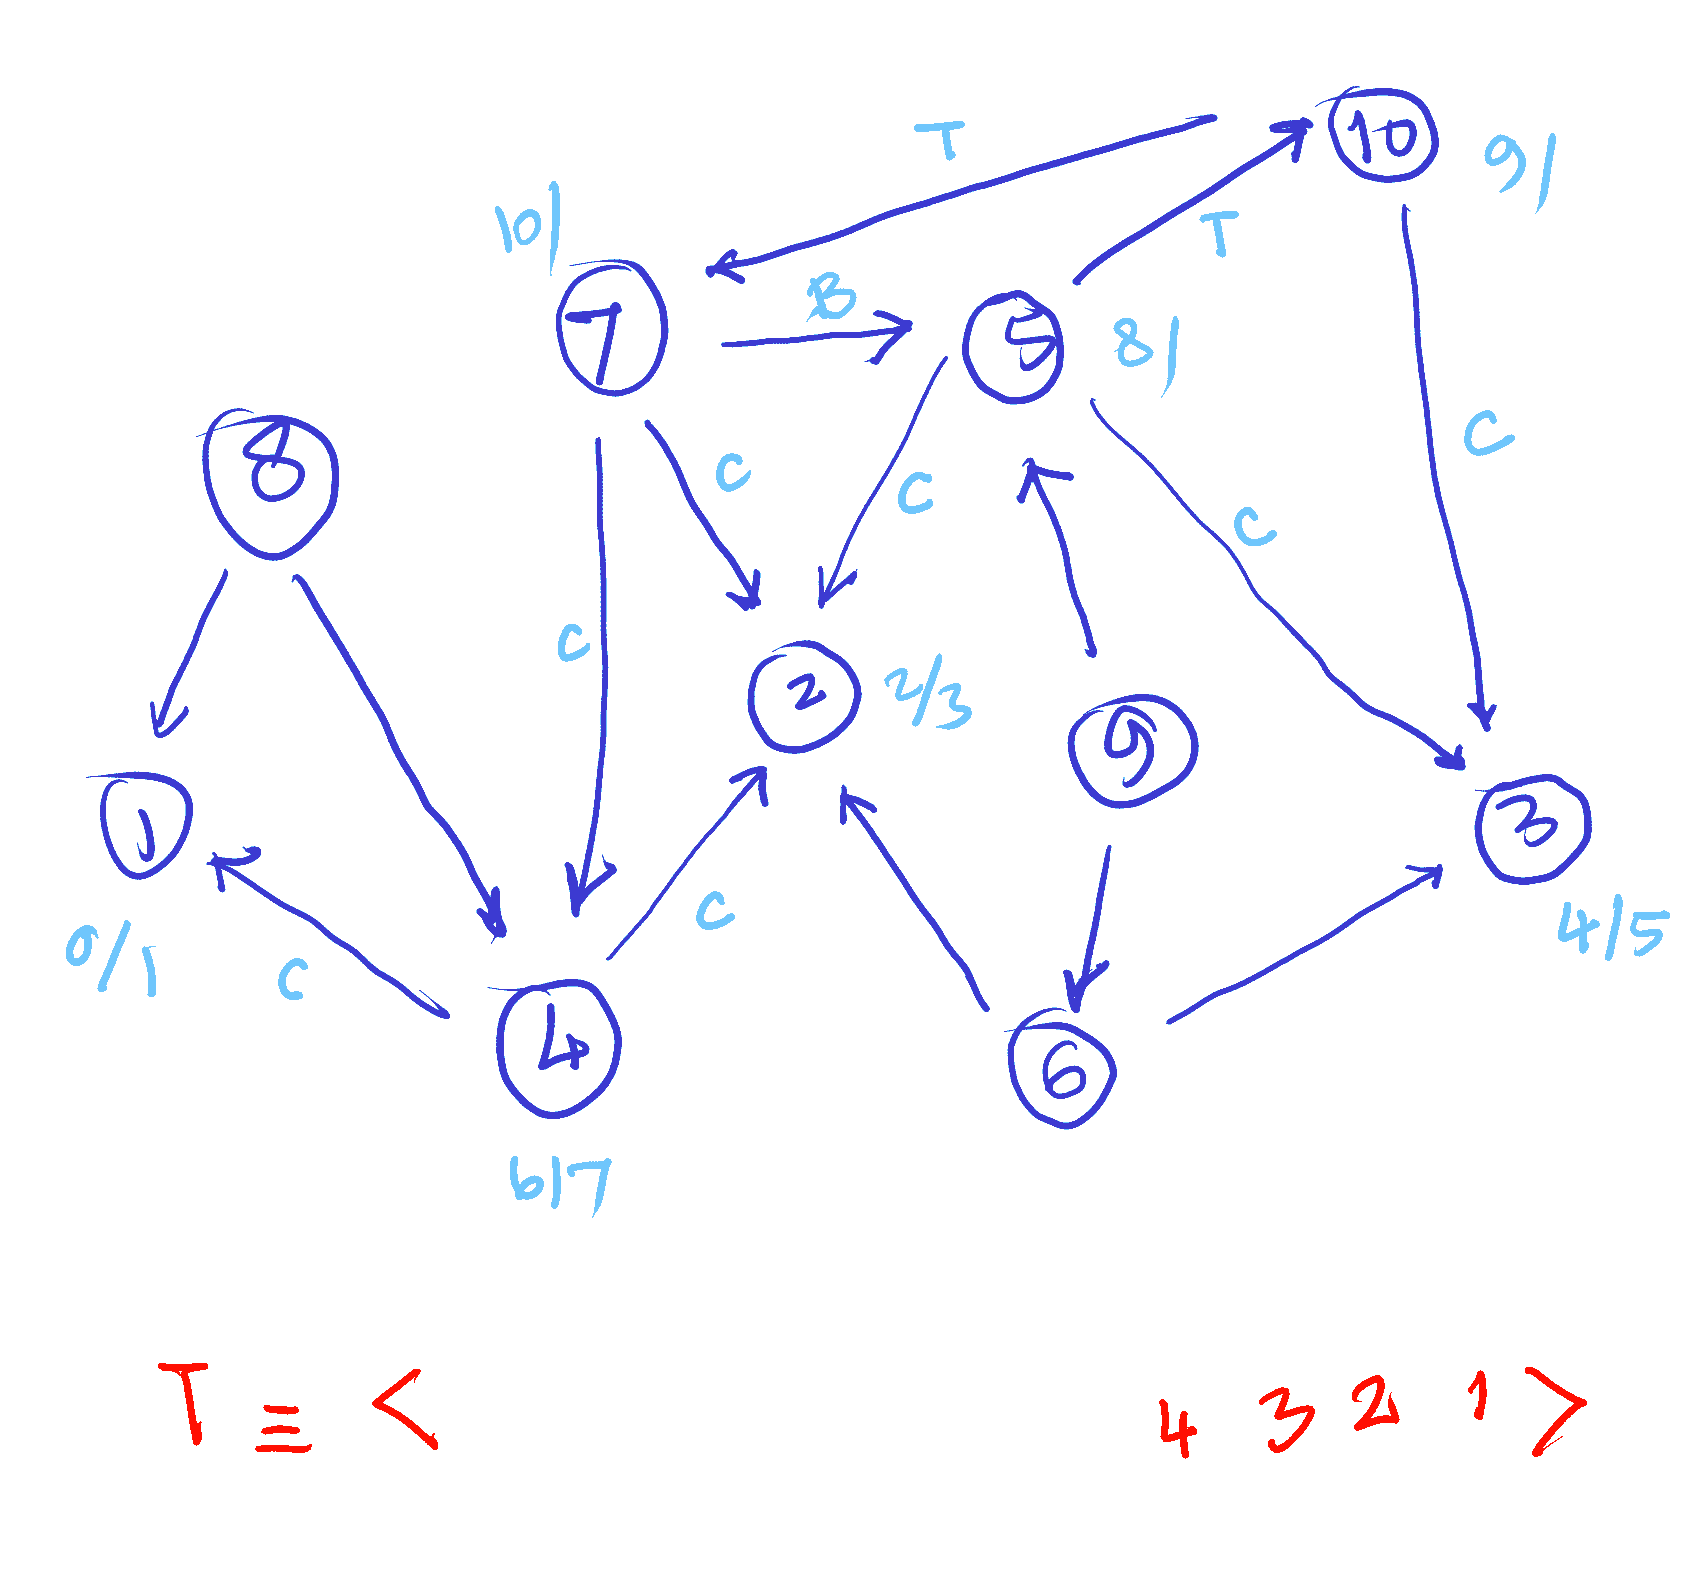
\includegraphics[width=.9\linewidth]{images/dfsOnDependencyGraph.png}
\caption{\label{fig:dfsOnDependencyGraph}DFS on Dependency Graph}
\end{figure}



\subsection{DFS Parenthesis Structure}
\label{sec:dfs-parenthesis-structure}
\paragraph*{Question}
\label{sec:org96310ef}

In DFS, discovery and finishing times are indicators of
ancestry.  Comment.

\paragraph*{Solution}
\label{sec:org600d85f}

\begin{enumerate}
\item When DFS discovers a vertex \(u\), it marks the
discovery time \(u\cdot d\) (the left parenthesis).
\item When DFS finishes visit to all the neighbours of
\(u\), it marks the finishing time \(u\cdot f\) (the
right parenthesis).
\item If \(u\) is an ancestor of vertex \(v\) in the DFS tree, then,
\begin{itemize}
\item \(u\) was discovered before \(v\), \emph{i.e.} \(u\cdot d <
     v\cdot d\);
\item The visit of \(u\) was finished after that of \(v\),
\emph{i.e.} \(v\cdot f < u\cdot f\); and
\item Thus, discovery/finish interval of \(u\) completely
encloses that of \(v\).
\end{itemize}
\end{enumerate}
\section{Problem Solving}
\label{sec:org07c09cd}

\subsection{Three jug problem}
\label{sec:org341c016}

\paragraph*{Question}
\label{sec:org1d3aefa}

There are three unmarked jugs \(A,B,C\) with a capacity
of 8, 5 and 3 units respectively.  Possible moves may
either empty a can into another or fill the other,
whichever occurs earlier.  Starting with \(A8,B0,C0\),
\textbf{determine algorithmically} if and how we can reach to
a split of \(A4,B4,C0\).

\begin{figure}[!h]
\centering
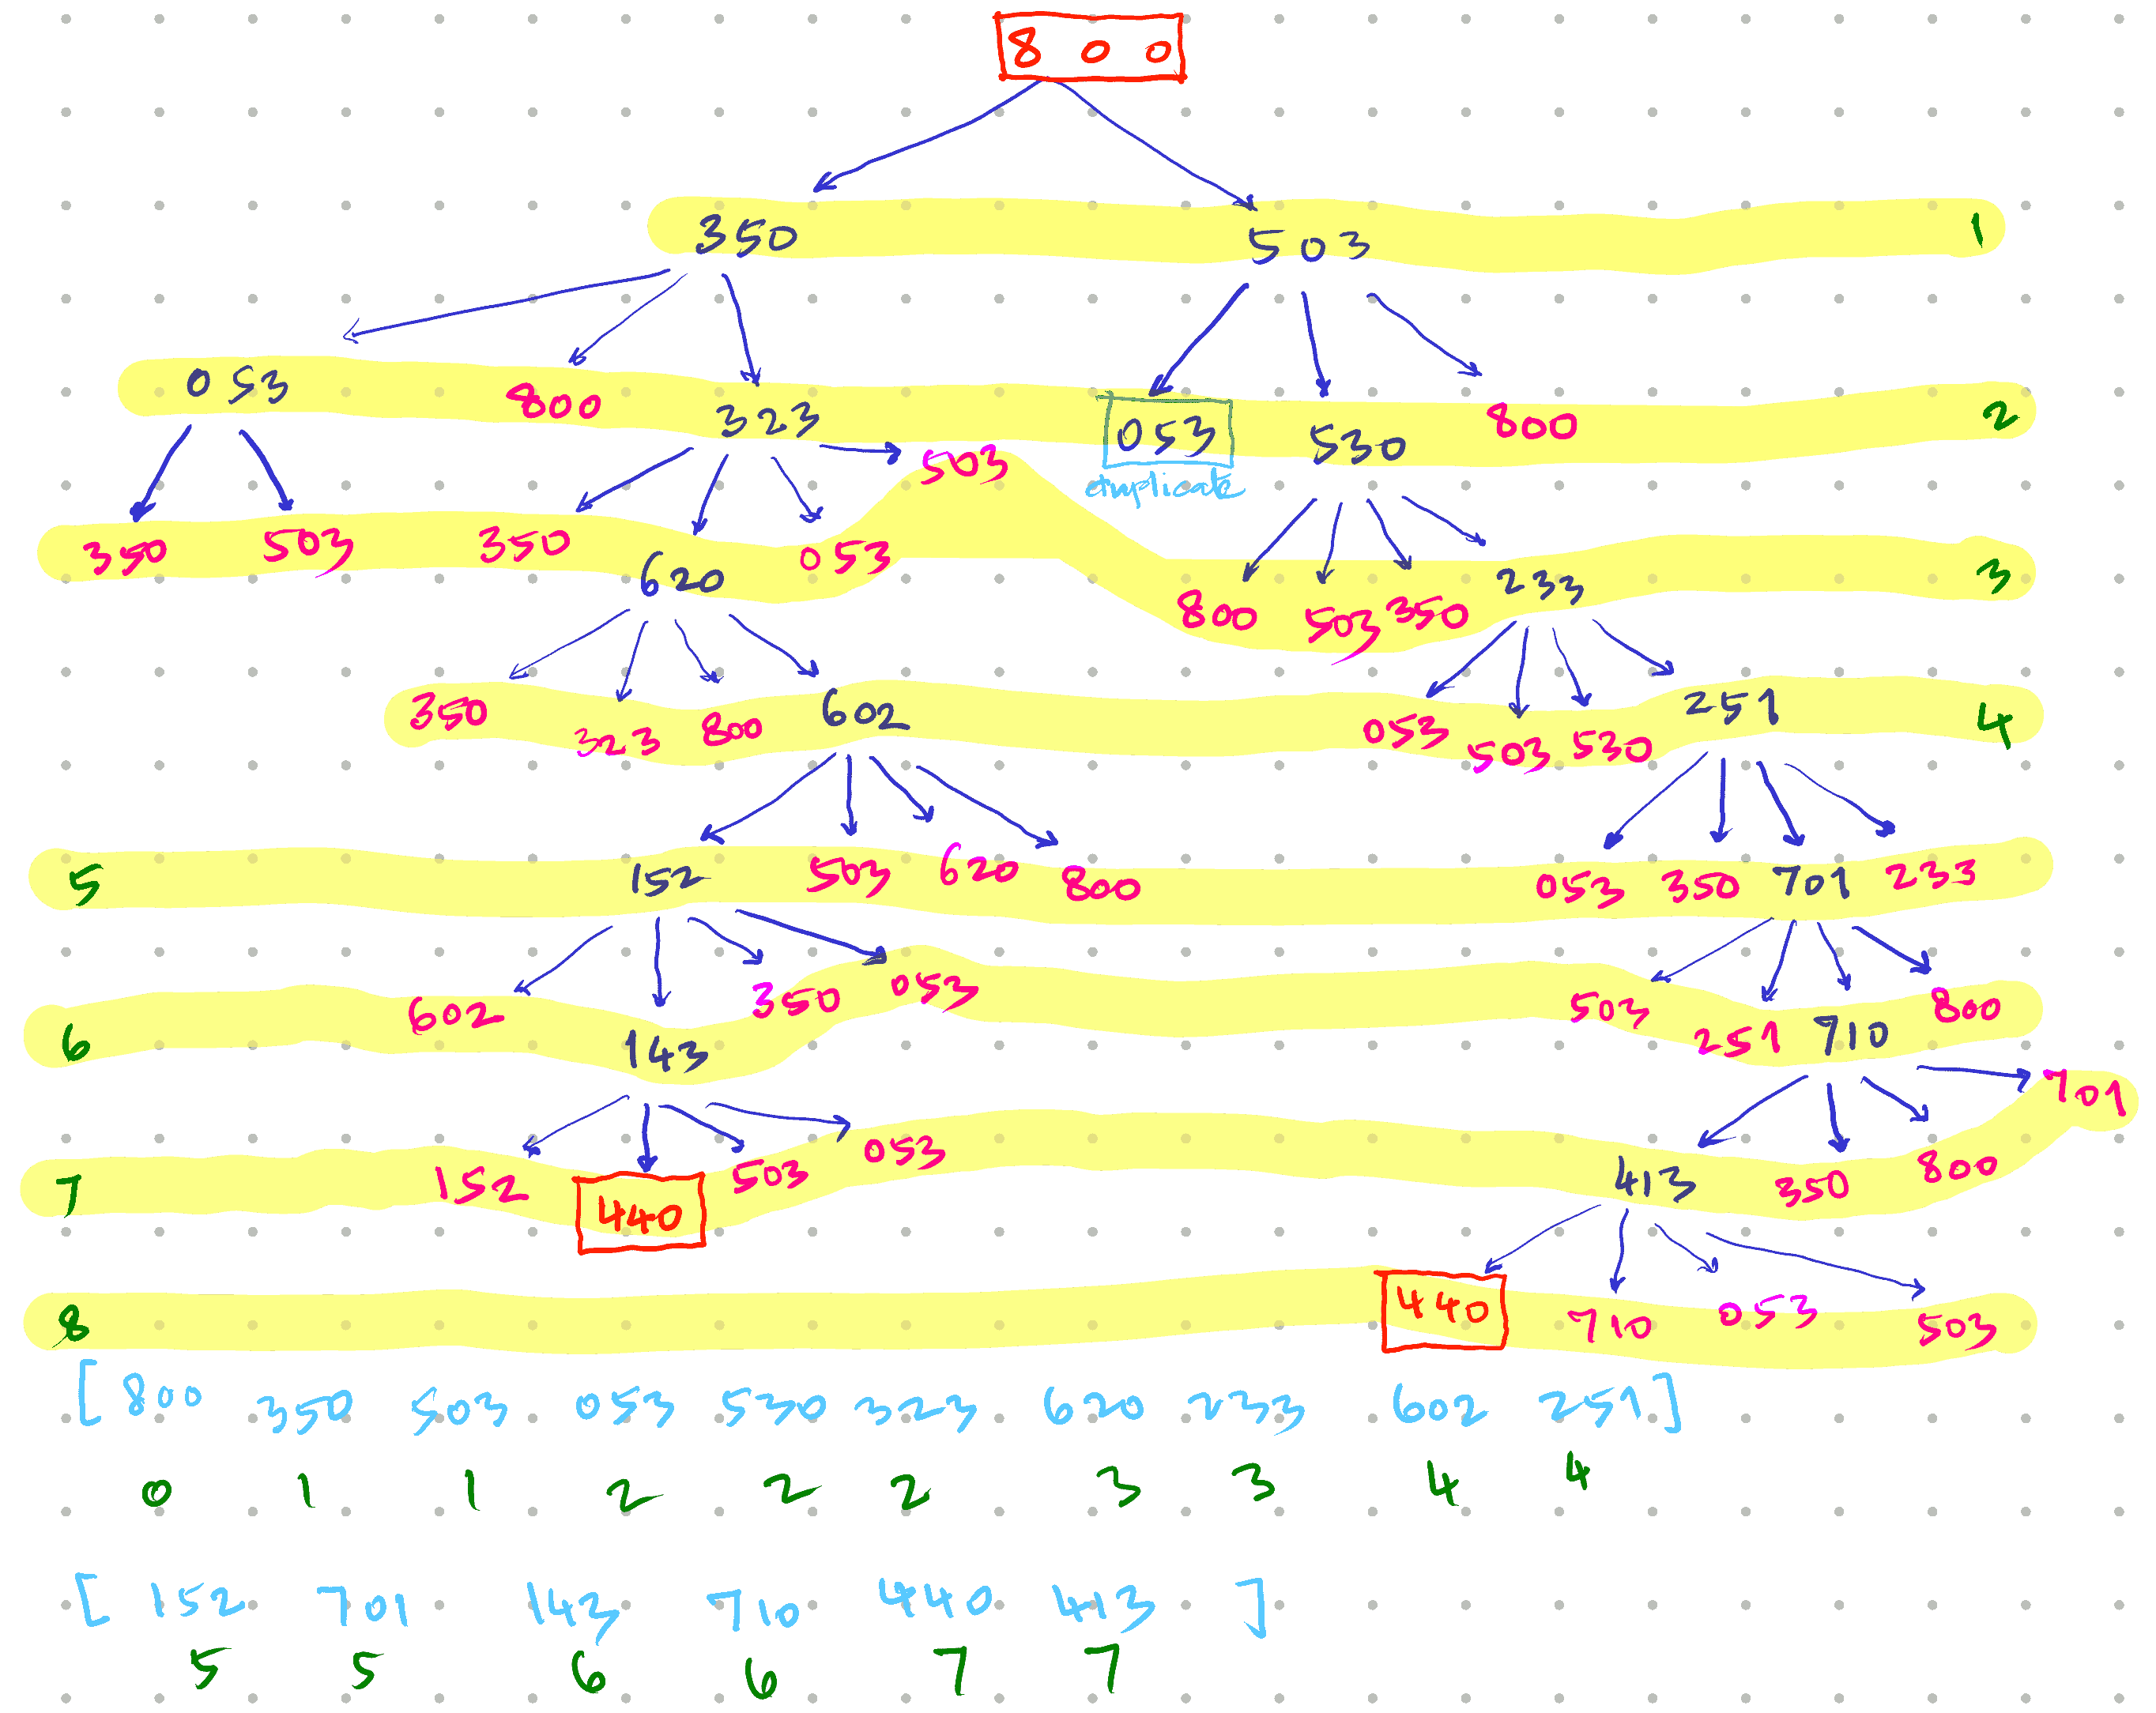
\includegraphics[width=.9\linewidth]{images/bfsOnStateGraph.png}
\caption{\label{fig:bfsOnStateGraph}BFS on State Graph}
\end{figure}

\paragraph*{Key Insight}
\label{sec:org86f692f}
\begin{enumerate}
\item The jugs are unmarked.  Hence, there is no way to
determine any intermediate quantity while pouring.
\item For every state reachable from any other state, at
least one of the jugs is either empty or full.  This
is a direct consequence of a \emph{possible move}
(action,) as defined in the problem.
\item Each jug may be poured into the other two, so there
may be 6 actions.  But at every state, at least one
jug is empty or full; the number of actions is
limited to 4.
\item Some moves are reversible, \emph{e.g.} \(A8,B0,C0
   \rightleftharpoons A3,B5,C0\).  As a consequence, the
resultant state graph is cyclic in nature.
\end{enumerate}

\paragraph*{Solution}
\label{sec:org0261f3c}

\begin{description}
\item[{State Space}] is a 3-vector \(\mathbf{v} \equiv
  Aa,Bb,Cc\) that satisfies,

\begin{align*}
\boldsymbol{0}
  \leqslant \begin{bmatrix}a&b&c \end{bmatrix}^{\top}
  & \leqslant \begin{bmatrix}8&5&3 \end{bmatrix}^{\top}
  \\
  a+b+c &= 8
\end{align*}

\item[{Start State}] \(\mathbf{s}=A8,B0,C0\)

\item[{Actions}] Pour from jug, until the latter is full,
or else empty the former.
\end{description}

Since the state graph is cyclic in nature, our solution
is based out of BFS. See 
Fig.~\ref{fig:bfsOnStateGraph}.

\subsection{Three jug problem 2}
\label{sec:org3b2338e}
\paragraph*{Question}
\label{sec:org4b419c4}
There are three unmarked jugs \(A,B,C\) with a capacity
of 8, 5 and 3 units respectively.  Possible moves may
either empty a can into another or fill the other,
whichever occurs earlier.  Starting with \(A8,B0,C0\),
can we can reach to a split of \(A4,B3,C1\).

\paragraph*{Solution}
\label{sec:org566cf5a}

\emph{(This is a logical deduction, not an algorithmic
solution.)}

From our key insights \emph{(earlier)},

\begin{quote}
For every state reachable from any other state, at
least one of the jugs is either empty or full.
\end{quote}

The state \(A4,B3,C1\) has neither of the jugs empty, nor
full!  \textbf{Hence this is not a reachable state!}
\end{document}
